\documentclass[10pt,a4paper,twopage]{article}

%for russian text
\usepackage[utf8]{inputenc}
\usepackage[english,russian]{babel}

%for links
\usepackage{hyperref}

%for images
\usepackage{graphicx}
\graphicspath{ {./images/} }
\usepackage{wrapfig}

%for margins and page dimensions
\usepackage[top=2cm, bottom=3cm, left=3cm, right=2.5cm]{geometry}
\usepackage{fancyhdr}
\renewcommand{\headrulewidth}{0pt}
\pagestyle{fancyplain}

%for table
\usepackage{array}

%for columns
\usepackage{multicol}
\setlength{\columnsep}{1cm}

%for spacing
\usepackage{setspace}

%headers and footers [odd]{even}
\lhead[]{}
\chead[]{}
\rhead[]{}
\lfoot[\textbf{\thepage}]{}
\cfoot[]{}
\rfoot[]{\textbf{\thepage}}

\title{Лабораторная работа №7. "Работа с системой компьютерной вёрстки TEX"}
\author{Маликов Глеб Игоревич}


\begin{document}
\maketitle

\section{Обязательное задание}
Сверстать страницу, максимально похожую на выбранную страницу из журнала "Квант".\\
Исходный файл \href{run:./source/Article1.gif}{Страница 1} \href{run:./source/Article1.gif}{Страница 2}\\
Результат \href{run:./Article.tex}{.tex} \href{run:./Article.pdf}{.pdf}

\section{Необязательное задание №1}
Сверстать титульный лист\\
Исходный файл \href{run:./source/Front.gif}{Тилутьный лист}\\
Результат \href{run:./Front.tex}{Front.tex} \href{run:./Front.pdf}{.pdf}


\section{Необязательное задание №2}
Используя пакет Beamer, необходимо сверстать 5 слайдов презентации с лекций по "Информатике".\\
Исходный файл \href{run:./source/Lecture.pdf#page=17}{Мера количества информации по Шеннону Слайды 17-21}\\
Результат\href{run:./Beamer.tex}{.tex} \href{run:./Beamer.pdf}{.pdf}

\clearpage
\hspace*{-1.2cm} 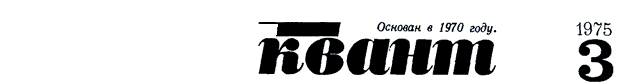
\includegraphics{lt1}
\vspace*{-1cm}
\begin{wrapfigure}[8]{l}{0.64\textwidth}
\hspace*{-0.4cm}
\includegraphics[width=0.68\textwidth]{lt2}
\end{wrapfigure}

\begin{spacing}{0.7}
\vspace*{0.1cm}
\noindent\textit{Научно-популярный\\
физико-математический\\
журнал\\
Академии наук СССР\\
и Академии педагогических\\
наук СССР\\}

\begin{wrapfigure}[4]{l}{0.7\textwidth}
\centering
\vspace*{-0.6cm}\hspace*{10.7cm}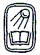
\includegraphics[width=0.07\textwidth]{lt3}
\end{wrapfigure}

\noindent\textit{Издательство«Наука»\\
Главная редакция\\
физико-математической\\
литературы\\}
\newline
\newline
\end{spacing}
\vspace*{-0.7cm}

\begin{wrapfigure}{l}{0.32\textwidth}
\begin{spacing}{0.9}
\noindent Главный редактор\\
\textit{академик} И. К. Кикоин\\
Первый заместитель\\
главного редактора\\
\textit{академик} А.Н. Колмогоров\\
\newline
\textbf{Редакционная коллегия:}\\
М. И. Башмаков,\\
C. Т. Беляев,\\
B. Г. Болтянский,\\
H. Б. Васильев,\\
Ю. Н. Ефремов,\\
B. Г. Зубов,\\
П. Л. Капица,\\
B. А. Кириллин.\\
\textit{главный художник}\\
A. И. Климанов,\\
C. М. Козел.\\
\textit{зам, главного редактора}\\
B. A. Лешковцев,\\
Л. Г. Макар-Лиманов,\\
A. И. Маркушевич,\\
H. А. Патрикеева,\\
И. C. Пстраков,\\
H. X. Розов,\\
A. П. Савин,\\
И. Ш. Слободецкий,\\
\textit{зам, главного редактора}\\
М. Л. Смолянский,\\
Я. А. Смородинский,\\
B. А. Фабрикант,\\
A. Т. Цветков,\\
М. П. Шаскольская,\\
C. И. Шварцбурд,\\
A. И. Ширшов.\\
\newline
\textbf{Редакция:}\\
B. Н. Березин,\\
A. Н. Виленкин,\\
И. Н. Клумова.\\
\textit{художественный редактор}\\
T. М. Макарова,\\
H. А. Минц,\\
Т. С. Петрова,\\
B. А. Тихомирова.\\
\textit{зав. редакцией}\\
Л. В. Чернова\\
\end{spacing}
\end{wrapfigure}

\begin{spacing}{0.5}
\hspace*{-1ex}\textbf{В НОМЕРЕ:}\\
\hspace*{3ex}\rule{9.5cm}{0.4pt}\\
\end{spacing}
\hspace*{-2ex}2 \textit{Н. Я. Виленкин, В. П. Лишевский.} Софья\\
\hspace*{3ex}Васильевна Ковалевская\\
12 \textit{И. И. Воробьев,} Электронный ветер\\
16 \textit{И. Н. Бронштейн.} Гипербола\\
25 \textit{И. П. Стаханов.} Масса и энергия в теории\\
\hspace*{3ex}относительности\\
30 \textit{Л. С. Хренов.} Средства вычислений\\
36 \textit{А. Б. Мигдал.} Письмо школьникам, которые хотят стать\\
\hspace*{3ex}физиками\\
\newline
\hspace*{3ex}\textbf{Математический кружок}\\
39 \textit{3. А. Скопец.} Расстояние между центроидами двух\\
\hspace*{3ex}систем точек\\
\newline
\hspace*{3ex}\textbf{Задачник «Кванта»}\\
44 Победители конкурса «Кванта»\\
46 Задачи М311-M315; ФЗ23 ФЗ27\\
48 Решения задач М273-М279; Ф285-Ф290\\
\newline
\hspace*{3ex}\textbf{Практикум абитуриента}\\
61 \textit{В. К. Егерен, А. Г. Мордкович.} Правильная\\
\hspace*{3ex}пирамида\\
66 \textit{Л. К. Белопухов, М. Г. Сухарев.} Московский институт\\
\hspace*{3ex}нефтехимической и газовой промышленности\\
\newline
69 \textbf{Спрашивайте - отвечаем}\\
\newline
\hspace*{3ex}\textbf{«Квант» для младших школьников}\\
71 Задачи\\
72 \textit{А. П. Савин.} Для чего нужны проценты?\\
\newline
74 \textbf{Ответы, указания, решения} \textit{(3-я стр. обложки)}\\
\newline
\hspace*{3ex}\textbf{Уголок коллекционера}\\
\hspace*{3ex}Смесь (с. 24, 35, 43, 68, 70).
\begin{spacing}{0.7}
\noindent\rule{9.5cm}{0.4pt}\\
\textit{
На первой странице обложки вы видите семейство кривых, координаты (x, y) точек которых удовлетворяют соотношению xy = k при всевозможных k>0. Эти кривые называются гиперболами. Подробнее о гиперболе и ее свойствах вы можете прочесть в статье на с. 16-24.}\\
\rule{9.5cm}{0.4pt}\\
\textit{
\copyright \hspace*{1ex} Главная редакция физико-математической литературы издательства «Наука», «Квант» №3, 1975 год}
\end{spacing}
\clearpage
\hspace*{-1.4cm}\noindent\rule{16.2cm}{0.4pt}\vspace*{1cm}\\
\begin{wrapfigure}[3]{l}{0.15\textwidth}
\vspace*{-1.7cm}\hspace*{1cm}
\includegraphics[width=0.15\textwidth]{l}
\end{wrapfigure}
\hspace*{1.5cm}\Huge\textbf{ Правильная пирамида}\\
\newline\vspace*{1cm}
\hspace*{1.5cm}\normalsize\textit{В. К. Егерев, А. Г. Мордкович}\\
\hspace*{-0.9cm}\noindent\rule{16.2cm}{0.4pt}\\
\vspace*{-0.7cm}

\begin{spacing}{1.1}
\begin{large}
\begin{multicols*}{2}
\noindent Решению многих геометрических задач присущ характер искусственности, что дало основание немецкому философу прошлого века Артуру Шопенгауэру бросить геометрии упрек в использовании «доказательств-мышеловок». Действительно, решение геометрических задач содержит мало шаблонов и часто производит впечатление фокуса. Тем более важно знать тот небольшой арсенал «стандартных» приемов, которые все-таки используются при решении этих задач. О некоторых приемах уже шла речь на страницах нашего журнала (см. например, статью И. А. Кушнир «Метод вспомогательного элемента», «Квант», 1974, № 2). В этой статье рассказывается еще об одном таком приеме.\\


\noindent\textbf{1. «Метод кастрюльки»}\\
Начнем с небольшой притчи. Андрею объяснили, как сварить яйцо: «Сними с гвоздя кастрюльку, налей туда воды, положи яйцо, зажги газ, поставь кастрюльку на газовую плиту и сними через 5 минут после того, как закипит вода». Андрюша так и сделал, все хорошо получилось. Но как-то, проснувшись утром, Андрей увидел, что вода в кастрюльку уже налита и газ горит. Подумав, он погасил газ, вылил воду и повесил кастрюльку на гвоздик, а затем сделал так, как его учили.\\
\indent Несмотря на кажущуюся несуразность такого поведения, метод возвращения к исходным данным задачи, которую мы умеем решать, является иногда наиболее рациональным. Назовем его «методом кастрюльки».\\

\noindent\textbf{2. Соотношения между углами в пирамиде}\\
На рисунке 1 изображена часть правильной п-угольной пирамиды SABCD…, SH-высота, SK-апофема. Введем следующие обозначения:

\leftskip=0.5cm
\noindent$\alpha$-угол между боковым ребром и плоскостью основания;\\
$\beta$-угол между боковой гранью и плоскостью основания;\\
$\gamma$-угол между смежными боковыми ребрами;\\
$\varphi$-угол между смежными боковыми гранями.

\leftskip=0cm
\vspace*{0.5cm}
\noindent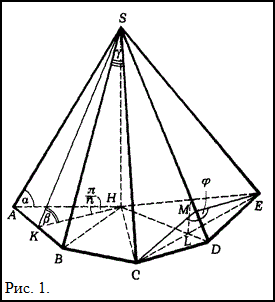
\includegraphics{fig1}
\end{multicols*}
\end{large}
\end{spacing}

\hspace*{-5ex}
\begin{tabular}{ c | c r| c | c }
\hline
Углы & \hspace*{0.7cm} Соотношения&& Область изменения углов & Связи между углами\\
\hline
&&&\\
$\alpha: \varphi$ & $\displaystyle \sin \alpha = \cot \frac{\varphi}{2} \cot \frac{\pi}{n}$ & (1)& $\displaystyle 0 < \alpha < \frac{\pi}{2}$ & \\
&&&\\
$\alpha: \gamma$ & $\displaystyle \cos \alpha = \sin \frac{\gamma}{2}/\sin \frac{\pi}{n}$ & (2)& $\displaystyle 0 < \beta < \frac{\pi}{2}$ & $\displaystyle \gamma < \pi - 2\alpha$ \\
&&&\\
$\alpha: \beta$ & $\displaystyle \tan \alpha = \tan \beta \cdot \cos \frac{\pi}{n}$ & (3)& $\displaystyle 0 < \gamma < \frac{\pi}{2}$ & $\displaystyle \alpha< \beta$ \\
&&&\\
$\beta: \gamma$ & $\displaystyle \cos \beta = \tan \frac{\gamma}{2}/\cot\frac{\pi}{n}$ & (4)& $\displaystyle \pi - \frac{2\pi}{n} < \varphi < \ \pi$ & \\
&&&\\
$\beta: \varphi$ & $\displaystyle \tan \beta = \frac {\sqrt{2} \cos \frac{\varphi}{2} } {\sqrt{-\cos \varphi - \cos \frac{2\pi}{n} } }$ & (5)& & $\displaystyle \varphi > \pi - 2\beta$ \\
&&&\\
$\gamma: \varphi$ & $\displaystyle \sin \frac{\gamma}{2} = \frac {\sqrt{-\cos \varphi - \cos \frac{2\pi}{n}}} {\sqrt{2} \cos \frac{\varphi}{2}}$ & (6)& & \\
\end{tabular}

\end{document}